% 项目导读（中文）：面向完全未接触过本项目的读者；数字与正式报告一致。
% 编译（LM2，两遍，目录 docs/report/stage_report_2/）：export PATH=/data6/jinxinhao/texlive/2026/bin/x86_64-linux:$PATH
%   xelatex summary_plain_zh.tex && xelatex summary_plain_zh.tex
\documentclass[11pt]{article}
\usepackage[margin=1in]{geometry}
\usepackage{amsmath,amssymb}
\usepackage{booktabs}
\usepackage{graphicx}
\usepackage{xcolor}
\usepackage{xeCJK}
\setCJKmainfont{FandolSong-Regular}[
  Extension = .otf, BoldFont = FandolSong-Bold,
  AutoFakeBold = 2.2, AutoFakeSlant = 0.2]
\setCJKsansfont{FandolHei-Regular}[Extension = .otf, AutoFakeBold = 2.2]
\renewcommand{\figurename}{图}
\usepackage[hidelinks]{hyperref}
\emergencystretch=3em

\title{\bfseries 把图像放大一倍，AI 就能看见将死的细胞了吗？\\[6pt]
\large ——阶段报告二导读（课程项目 bdd26）}
\author{}
\date{2026 年 10 月 1 日}

\begin{document}
\maketitle

\section*{背景：上一份报告留下了两个猜想}

上一阶段的结论（见阶段报告一导读）：AI 在病理切片上找细胞核，最难的一类是\textbf{凋亡核}
——细胞死亡后留下的皱缩、碎裂、深染的残迹——近五年所有已发表模型在这一类上的得分都停留
在 0.13--0.19，其它类别一般在 0.4 以上。逐项拆解错误后我们确认：问题不是“认错”，而是
“看不见”（约 38\% 的凋亡核完全没有被检出），而且换了数据、换了训练技巧都无济于事。

当时留下两条没来得及检验的出路，本阶段的全部工作就是把它们验完：

\begin{enumerate}
\item \textbf{换一种架构。}常见的模型是“先给每个像素打分、再把相邻的像素围成核”（下称
      “描边派”）。另一派“找点派”先预测每个核的中心点、再围绕点组装轮廓——论文里报出的
      凋亡核成绩，恰恰是找点派里最亮眼的（一个叫 KongNet 的模型）。
\item \textbf{把图像放大。}凋亡核个头小（面积中位数只有普通核的约三分之一），256 像素的
      工作分辨率下每个核只占十几个像素——也许模型不是不会认，是根本看不清。
\end{enumerate}

按事先约定的严格标准（官方三折划分数据；参数只在验证部分上调；测试部分只评一次；每个结论
用多个随机种子重复），两条猜想的答案都出来了。

\section*{发现一：换“找点派”架构，不仅没更好，反而差了 11 分}

KongNet 的作者公开了三份分别训练的模型权重，但没有说明哪份对应数据的哪个划分。我们先解决
了这个问题：把每份权重在数据的三个部分上各测一遍，看它在哪部分“记得最牢”——训练过的数
据上成绩会明显偏高，据此就能对号入座，全程不碰测试数据。

之后按严格标准复评：KongNet 的整体得分只有 0.346，比我们测过的“描边派”里\emph{最弱}的
还低 11 分；文献里最亮眼的凋亡核成绩（$F_c$ 0.59），在我们的口径下只剩 0.34。

失败的方式很能说明问题：\textbf{挨在一起的同类核被“粘”成一坨}。它把互相接触的核合并的
比例是描边派模型的三四倍——而凋亡核恰恰经常以“碎块群”的形态出现（核碎裂，karyorrhexis）。
也就是说，凋亡核的困难一半在“找不到”，另一半在“找到了却分不开”，而找点派的组装方式把
“分不开”变得更糟。结论：这不是架构流派能解决的问题。

\section*{发现二：另一个更强的模型，也兑不出凋亡核的收益}

我们又复评了 LKCell-L——公开权重的模型里整体成绩最好的一档（论文 0.508）。两个发现：

\begin{itemize}
\item 它比论文\textbf{均匀地}低约 1.5 分：每项指标都低这么多。这种“整体平移”说明差异来
      自评测流程（选哪个存档点、怎么调后处理），不是我们测错了。
\item 在同等条件下，它勾轮廓确实更准（不分类别的分割得分更高），但\textbf{认类型更差}，
      凋亡核得分反而比我们自己的基线低 2.2 分。它找凋亡核的能力其实更强——找到的核却过
      不了“类型配对”这一关，还是换不成凋亡核得分。
\end{itemize}

两个模型合起来给出同一句话：\textbf{模型整体的强弱，和解决凋亡核，是两回事。}

\section*{发现三：把分辨率放大一倍，凋亡核确实好了——但要付一笔明码标价}

这是本阶段的主结果，过程像一次侦探破案。

\paragraph{第一步：放大。}把工作分辨率从 256 像素倍增到 512，其它一切（模型、训练配方、
数据）都不动。结果：事先登记的凋亡核指标\textbf{全部}变好——图内部的凋亡核漏检率从
35\% 降到 25\%，连最难的子宫脱落细胞团都从 0.041 升到 0.055。但整体分数全面下降
1.8--2.6 分（依指标）。按事先定的“凋亡核改善且整体不退步”标准：失败。

\paragraph{第二步：钱丢在哪了？}三个证据锁定了位置。其一，下降与凋亡核的改善\emph{不在
同一批图上}——凋亡核变好的图整体分数基本没动，丢分的图恰恰是不含凋亡核的。其二，把核按
大小分层（图~\ref{fig:zhsize}）：200 像素以下的小核\textbf{全部}变好（凋亡核也不例外），
核越大掉得越多——受损的是\emph{大核}，与类别无关。其三，被正确匹配的核，轮廓质量完全没
变。大核不是被认差了，是\textbf{被切碎了}：一个核被切成最多 7 块的“马赛克”，而外轮廓
还贴着标准答案（图~\ref{fig:zhmontage}）。

\begin{figure}[ht]
\centering
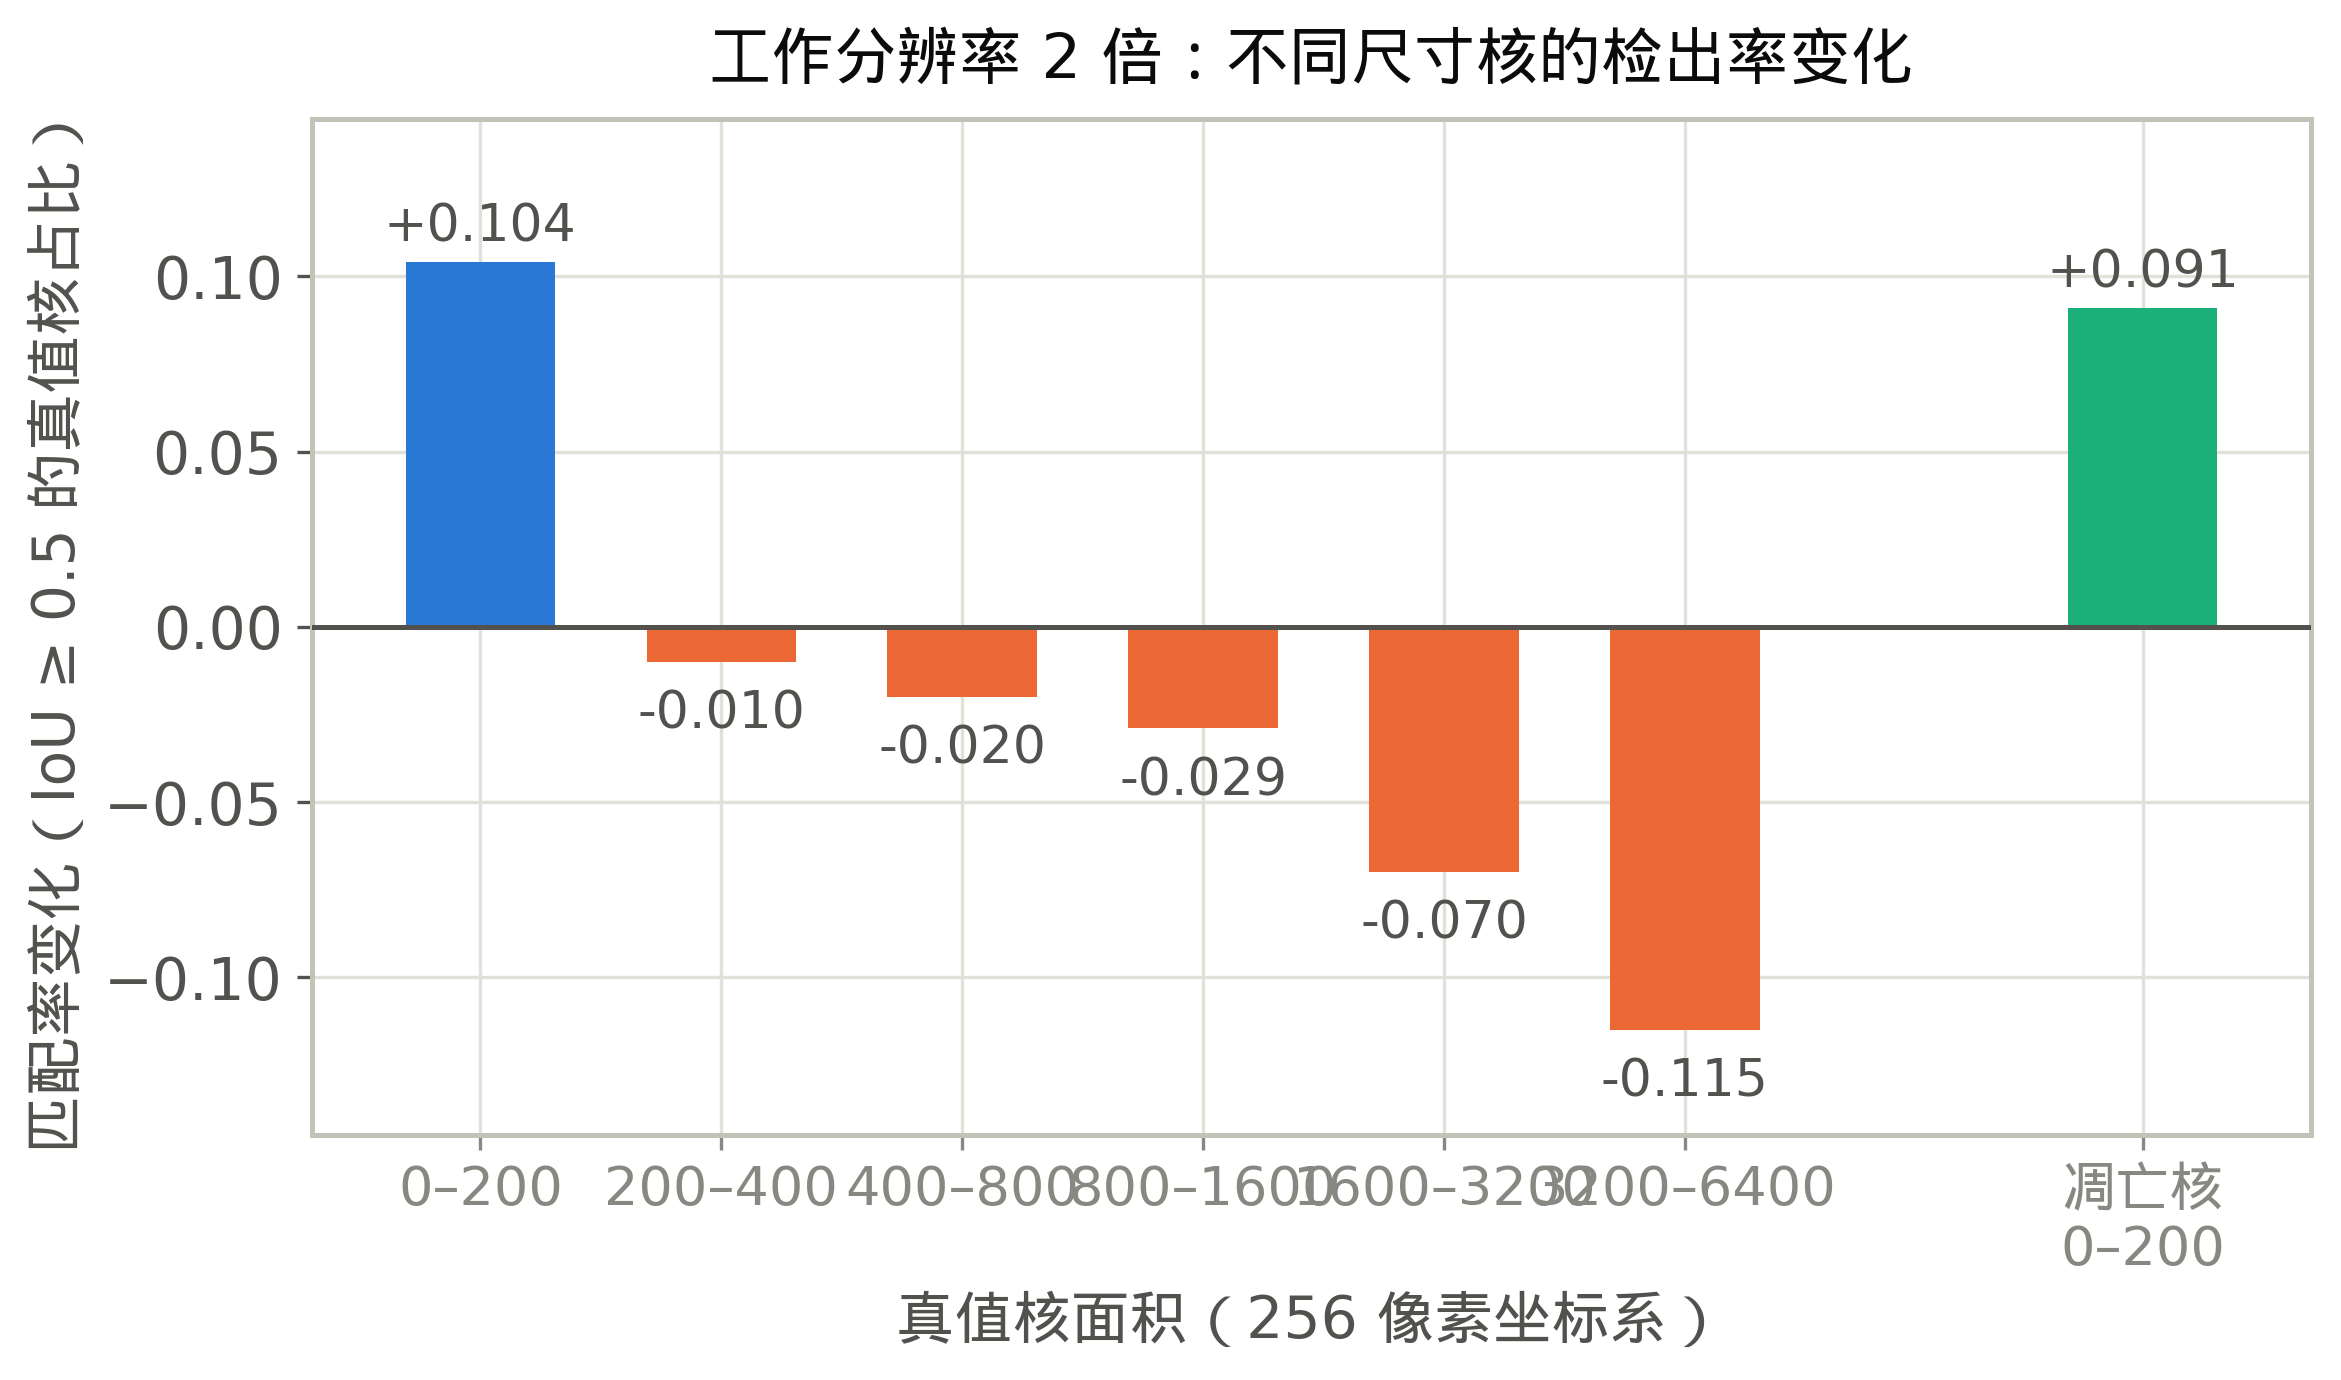
\includegraphics[width=0.9\linewidth]{figs/chart_size_bins_zh.png}
\caption{分辨率倍增后各尺寸核的检出率变化：小核全赢，大核全输，单调过渡——问题的坐标轴
是核的\emph{大小}，不是核的\emph{类别}。}
\label{fig:zhsize}
\end{figure}

\begin{figure}[ht]
\centering
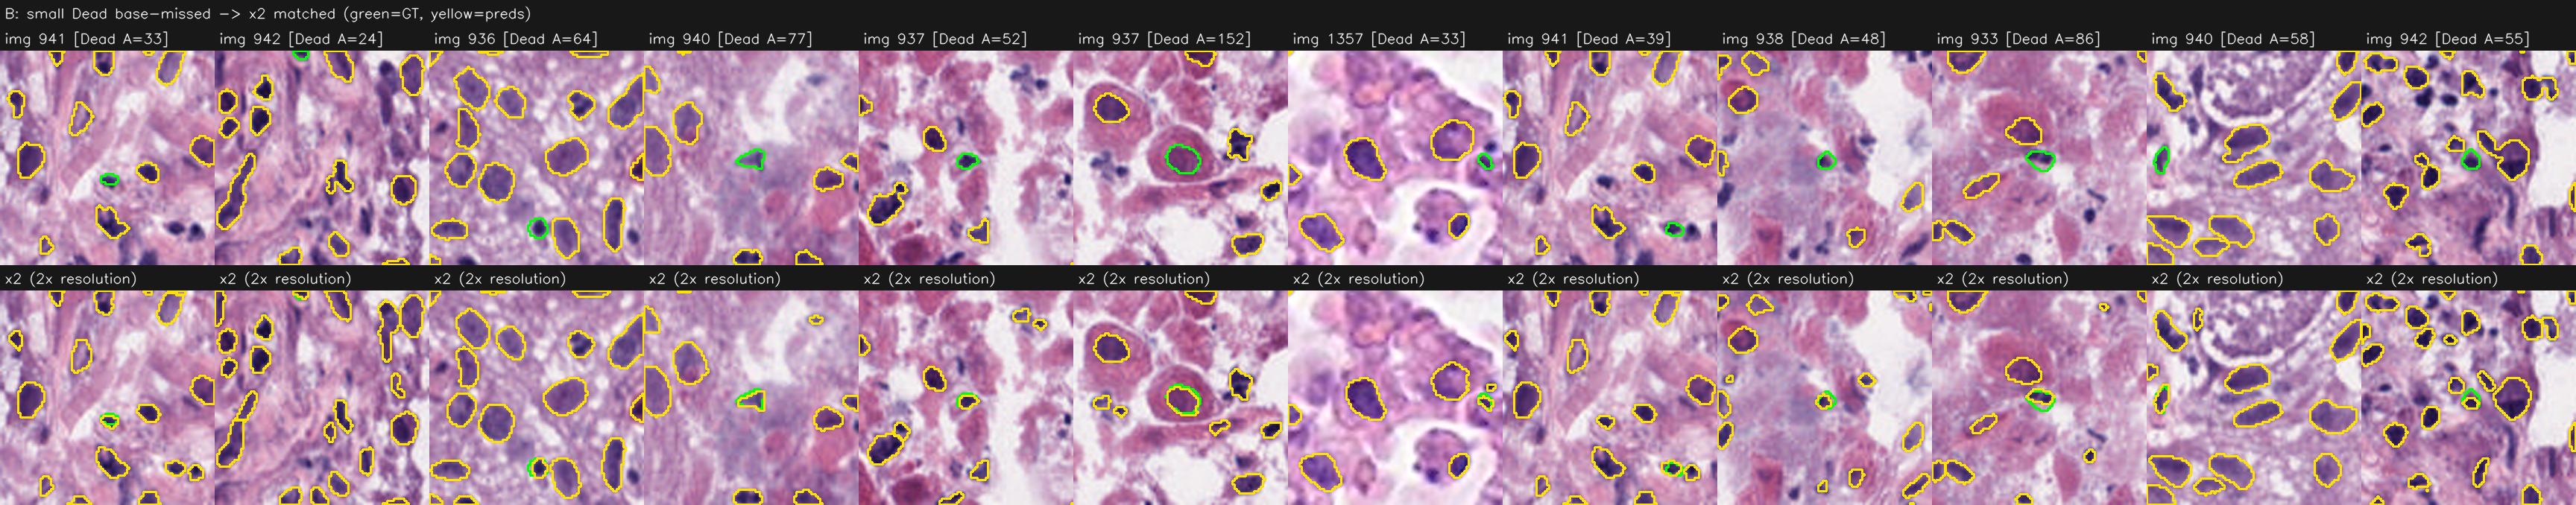
\includegraphics[width=\linewidth]{figs/x2_montage_gain.png}\\[2pt]
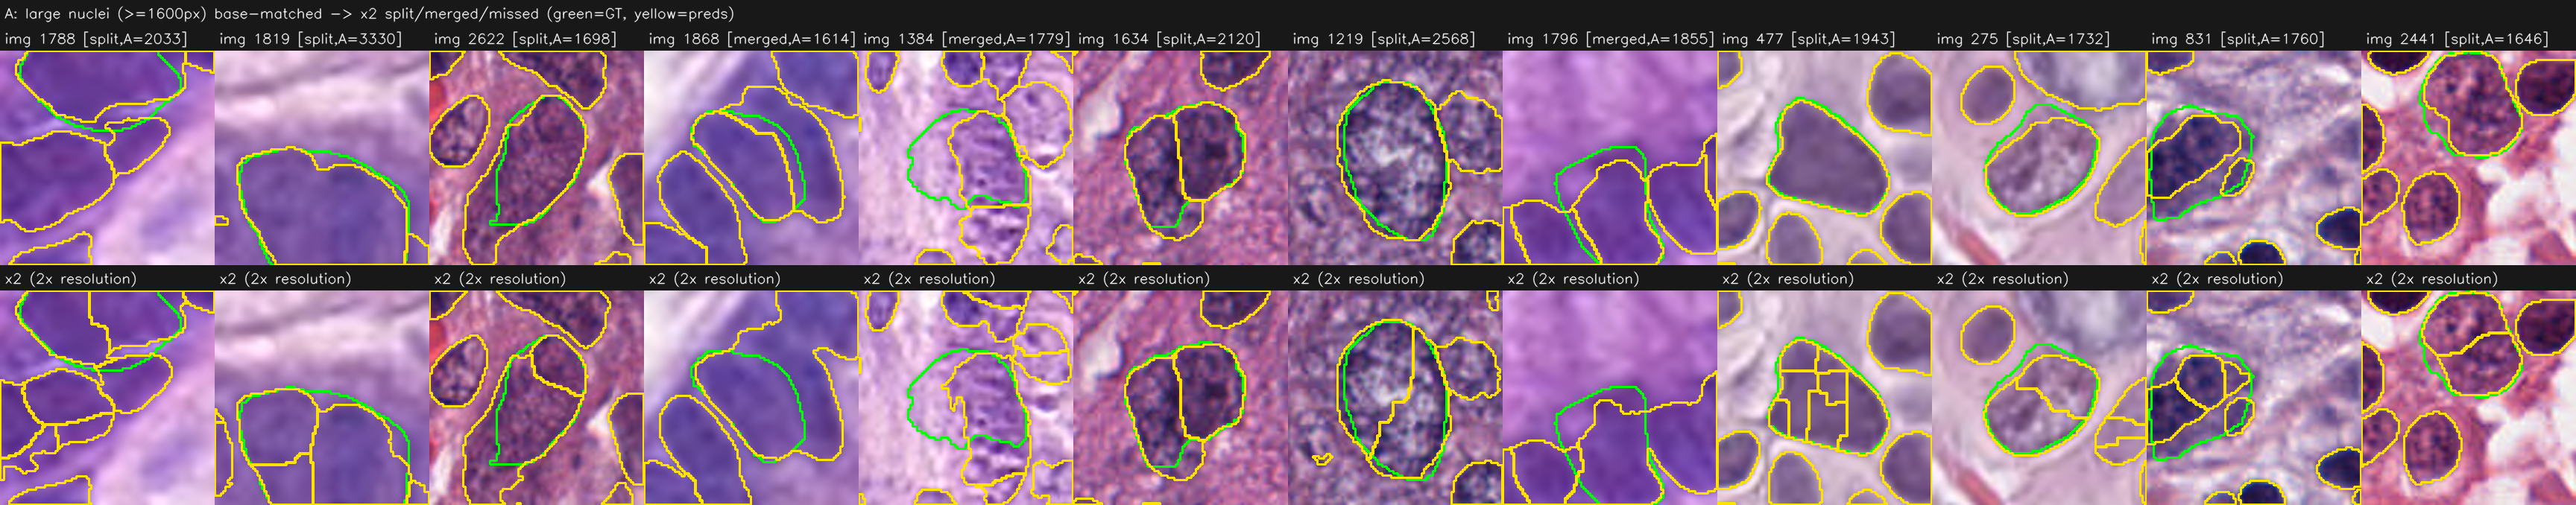
\includegraphics[width=\linewidth]{figs/x2_montage_damage.png}
\caption{上排对比（增益）：绿色是人工标注，黄色是模型预测——256 分辨率下没有任何预测
（上行），512 下被正常检出（下行）。下排对比（损伤）：256 下作为完整单体检出的大核（上
行），512 下碎成一堆小块（下行），但外围轮廓仍然贴着标注。}
\label{fig:zhmontage}
\end{figure}

\paragraph{第三步：真凶是两个写死的数字。}“把 512 的预测图缩回 256 时丢了信息”是最直观
的嫌疑，但被“匹配核轮廓质量不变”排除了。顺着线索查到模型后面的经典后处理代码：分水岭解
码里有两个\textbf{按像素单位写死}的常数——面积小于 10 平方像素的目标一律丢弃、边缘提取算
子的窗口宽度固定为 21 像素。分辨率放大一倍后，这两个门槛在\emph{真实物理尺寸}上悄悄减半：
本该被滤掉的细碎噪声活了下来、把大核切开；本该被合并的碎片漏进了预测列表。整个领域几乎
都在用这套继承自 HoVer-Net 的后处理代码，这个坑此前没有文献指出过。

\paragraph{第四步：修复，以及一个“杠杆”。}修复方案在动手前就登记：把两个常数按倍数缩放
（10$\times$4、21$\times$2）。改两行代码，代价收回 50--87\%（依指标不同），凋亡核增益分毫
未损、还略增。接着再加一个只在验证数据上选好的小杠杆——把切碎的\emph{同类}相邻块合并回
去、丢掉贴着图边界的细条——在全部 9 次重复实验（3 个数据划分 $\times$ 3 个随机种子）
上都取得严格变好的成绩。

\paragraph{第五步：诚实的终局。}最后一次大考是 $3\times3$ 的划分 $\times$ 种子网格
（图~\ref{fig:zhgrid}），判定标准事先写好。结果一分为二：

\begin{itemize}
\item \textbf{代价是稳健的}：整体分数下降在每一次重复中方向一致，幅度约是随机波动
      （换随机种子重训带来的差异）的 5 倍——真效应。
\item \textbf{凋亡核增益是脆弱的}：折算下来只有随机波动的 0.4--0.7 倍，五次同种子配对比较
      里输了一场，有一个数据划分的种子均值甚至翻负。
\end{itemize}

\begin{figure}[ht]
\centering
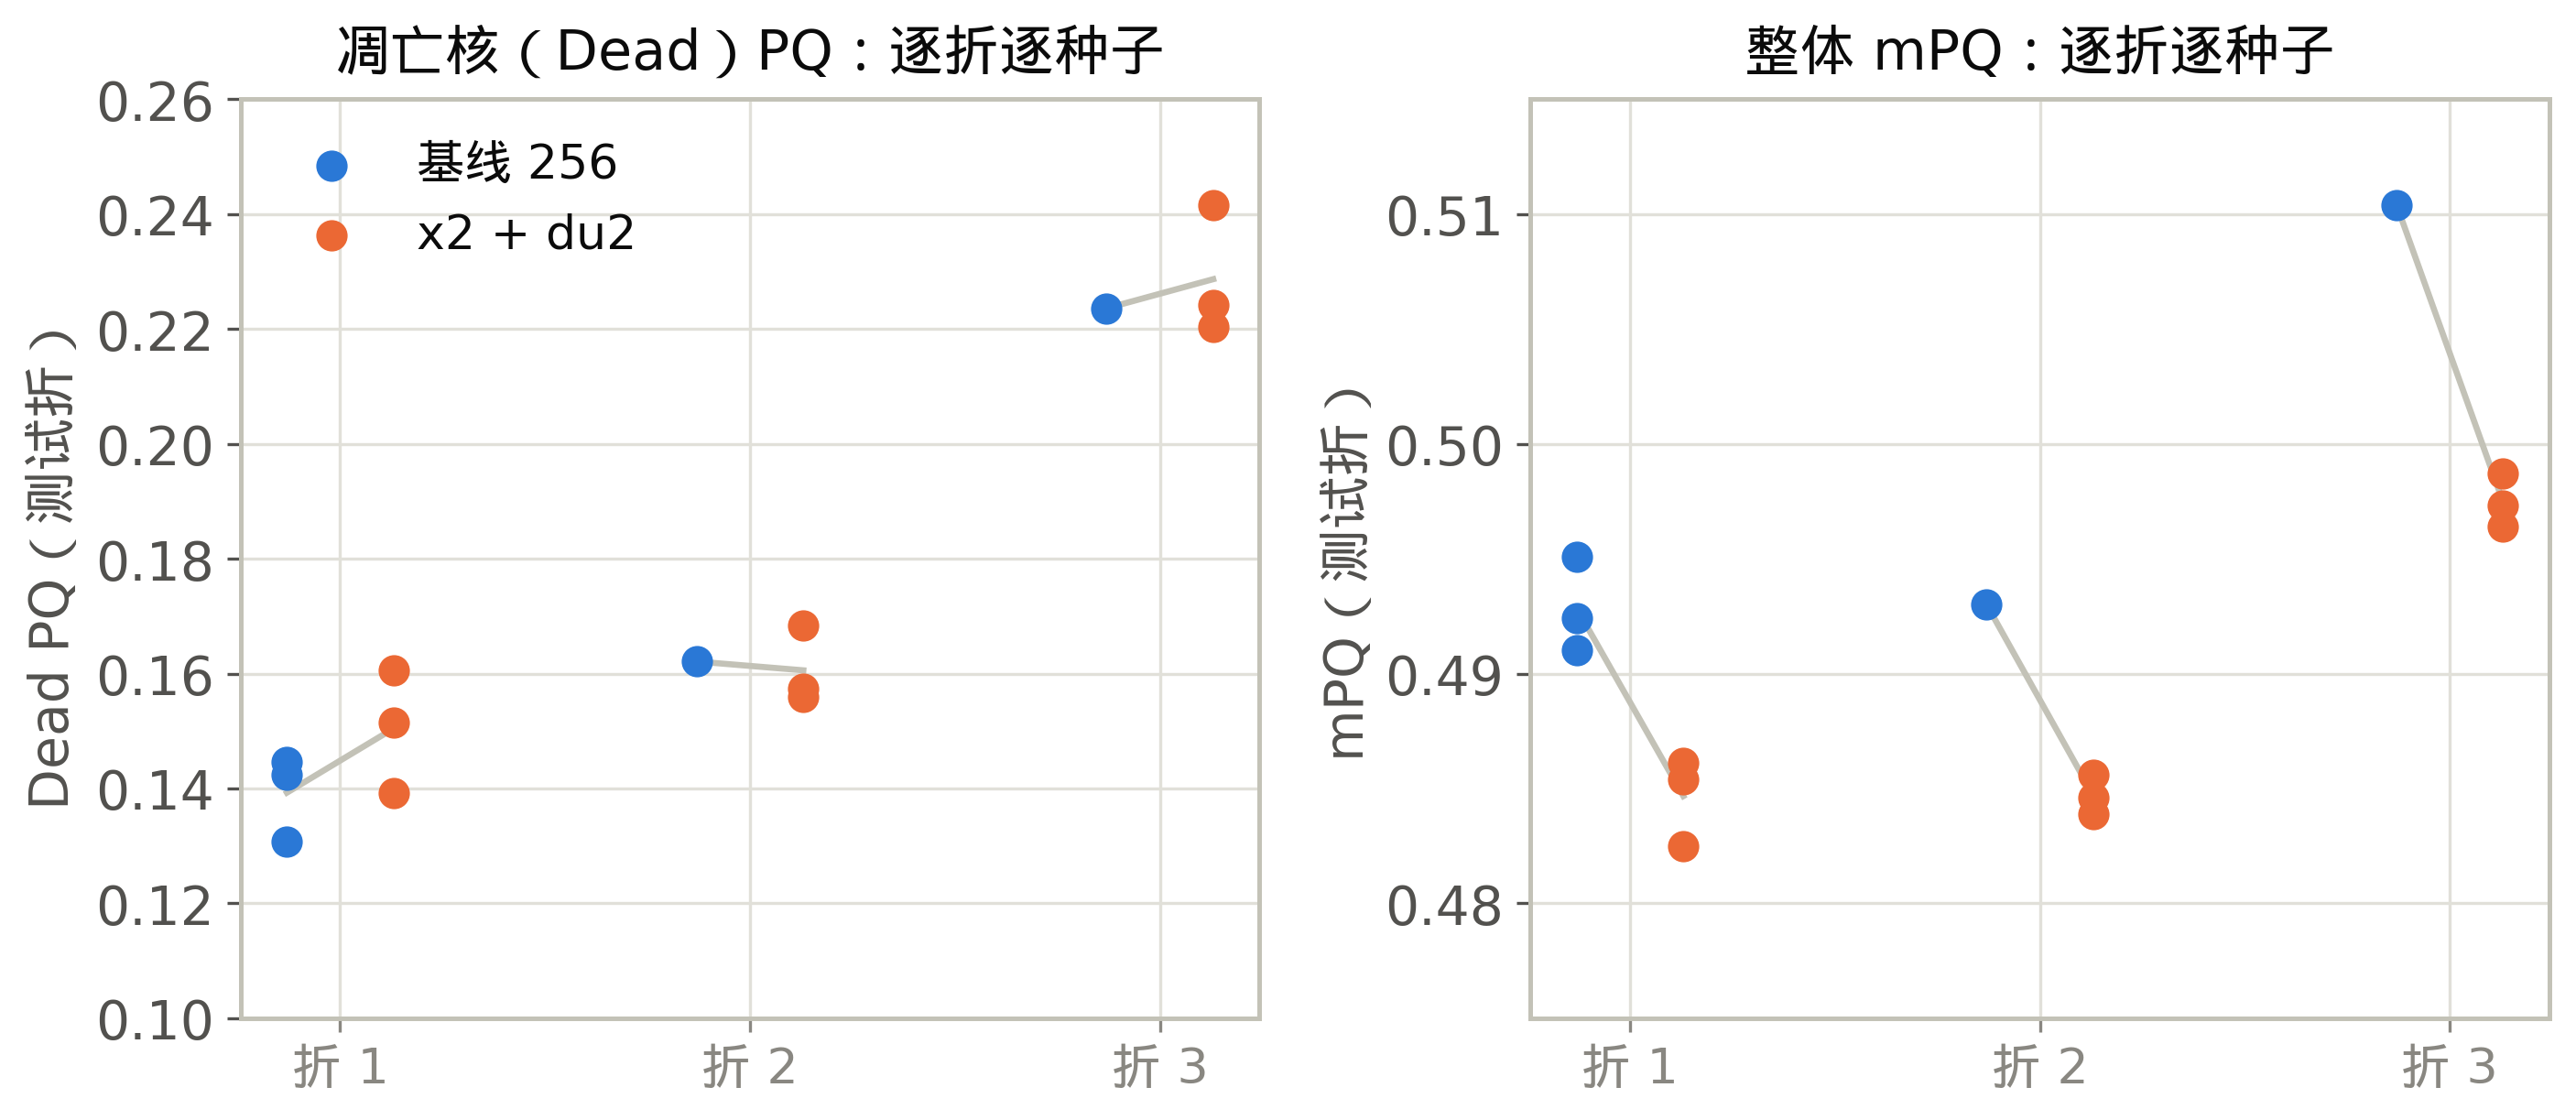
\includegraphics[width=0.98\linewidth]{figs/chart_seed_grid_zh.png}
\caption{种子网格：3 个数据划分 $\times$ 3 个随机种子。右图整体分数——橙点（512 分辨率）
每次都低于蓝点（基线），代价确凿；左图凋亡核分数——橙蓝交错，有一个划分上橙色均值反而
更低，增益脆弱。}
\label{fig:zhgrid}
\end{figure}

所以最终答案是：\textbf{放大一倍确实让 AI“看见”了更多将死的细胞}（漏检率降 7 个百分点，
这一项在所有重复中方向一致），但它不是免费的：要付出约 0.8 分的整体分数。这是一次明码标
价的交换，是否值得取决于下游更在乎哪一头；而“凋亡核类得分提高 0.5 分”这种头条数字，在
这项基准的噪声水平下不足为凭——我们同时报告了哪个数字可信、哪个不可信。

\vspace{1.5em}
\noindent\rule{\linewidth}{0.4pt}

\vspace{0.5em}
\noindent{\small 本文是《阶段报告二》的导读。完整的数字、表格与文献见同目录下的正式报告：\\
中文版 \texttt{stage\_report\_2\_zh.pdf}，\ 英文版 \texttt{stage\_report\_2.pdf}；\\
上一阶段的背景见 \texttt{../stage\_report\_1/summary\_plain\_zh.pdf}。}

\end{document}
